\documentclass[conference,harvard,brazil,english]{sbatex}
\usepackage[utf8]{inputenc}
\usepackage{ae}
%
% LaTeX2e class SBATeX
%
%
% Versão para Overleaf 
% Diego Eckhard
% diegoeck@ufrgs.br
%
%
% Versão 1.0 alpha
%   Walter Fetter Lages
%   w.fetter@ieee.org
%
% Este arquivo sbai2013.tex é uma adaptação do arquivo revista.tex,
% Versão: 1.0 alpha, desenvolvido por Maurício C. de Oliveira,
% mcdeoliveira@ieee.org.
%
% As adaptações fazem com que, por default, sejam utilizadas
% as opções adequadas para o formato do SBAI 2017.
% --------------------------------------------------
%  Estes comandos são necessários apenas para a
%  a geração deste artigo exemplo. Eles não fazem
%  parte do estilo SBATeX.
% --------------------------------------------------
\makeatletter
\def\verbatim@font{\normalfont\ttfamily\footnotesize}
\makeatother
\usepackage{amsmath}
% --------------------------------------------------

\usepackage{graphicx}
\usepackage{float}

\usepackage[lined,ruled,boxed]{algorithm2e}
%\usepackage{algorithmic}



\usepackage[table]{xcolor}
\usepackage{booktabs}

\usepackage{caption}
\usepackage{subcaption}

\usepackage{url}


%-----------------------
\usepackage{mathtools, nccmath}
\newcommand{\N}{\mathbb N}
\newcommand{\Q}{\mathbb Q}
\newcommand{\R}{\mathbb R}

\usepackage{xparse}
%
\DeclarePairedDelimiterX{\set}[1]{\{}{\}}{\setargs{#1}}
\NewDocumentCommand{\setargs}{>{\SplitArgument{1}{;}}m}
{\setargsaux#1}
\NewDocumentCommand{\setargsaux}{mm}
{\IfNoValueTF{#2}{#1} {#1\,\delimsize|\,\mathopen{}#2}}%{#1\:;\:#2}

\parindent = 0pt

\usepackage{amsfonts}
\newcommand{\commentib}[1]{{\color{blue} [IB: #1]}}

\begin{document}

% CABEÇALHO

\title{PLANNING AND UAV MISSION EVALUATION FOR INTRALOGISTICS PROBLEM}

\author{Thiago Cavalcante}{thiagorodrigoengcomp@gmail.com}
\address{Graduate Program in Electrical and Computer Engineering, Federal University of Amazonas, Manaus, AM, Brazil}

\author{Iury Bessa}{iurybessa@ufam.edu.br}
\address{Department of Electricity, Federal University of Amazonas, Manaus, AM, Brazil}



% \twocolumn apenas para conference
\twocolumn[

\maketitle

\selectlanguage{brazil}
\begin{abstract}
 Este artigo apresenta o desenvolvimento de planejadores de missão na intralogística para um veículo aéreo não tripulado comercial, equipado com uma garra robótica, em um ambiente industrial onde há almoxarifado de insumos, linhas de produção e deposito de produtos. Neste trabalho, o planejador gera comandos necessários para realizar uma missão a qual compreende desde a entrega de insumos trazidos do almoxarifado à linha de produção, até a entrega do produto final ao cliente. Foram desenvolvidas duas abordagens diferentes para planejamento de missão: na primeira abordagem, utilizou-se uma simples heurística que resolve o problema; já na segunda abordagem, utilizou-se uma técnica com escalonamento de tarefas (processo de produção). Estas abordagens seguem algumas regras de produção que serão apresentadas ao longo deste trabalho. Foi realizado uma avaliação dos planejadores de missão desenvolvidos, verificando o custo de ambos, realizando algumas medidas de tempo de execução, bem como comparando estes resultados com o custo ótimo obtido  com a ferramenta de otimização CPLEX.   \end{abstract}

\keywords{Planejamento de Missão, Sistemas de Manufatura.}

\selectlanguage{english}
\begin{abstract}
 This paper presents the development of mission planners in intralogistics for a commercial unmanned aerial vehicle equipped with a robotic gripper in an industrial environment where there are a warehouse of inputs, production lines and a product warehouse. In this work, the planner generates the necessary commands to carry out a mission that includes everything from the delivery of inputs brought from the warehouse of inputs to the production line until the final product is delivered to the customer (product warehouse). Two different approaches were developed for mission planning: in the first approach, a simple heuristic was used to solve the problem; in the second approach, a technique with task scheduling (production process) was used. These approaches follow some production rules that will be presented throughout this work. An evaluation of the mission planners developed was performed, verifying the cost of both, performing some measures of execution time, as well as comparing these results with the optimum cost obtained with the IBM ILOG CPLEX optimizer.
\end{abstract}

\keywords{Mission Planning, Manufacturing Systems.}
]

% CONTRIBUIÇÃO
\selectlanguage{english}

\section{Introduction}
\label{sec:introduction}

% Use of a commercial UAV - 3DR IRIS + in the intra-logistics, {\it i.e., Internal Logistics of movement and storage.}, aiming to give another option of agility in the manufacturing process. Additionally, it will be approached a study of evaluation of the cost of the missions that the UAV executes in this process.

Logistics has become a competitive and fundamental factor for organizations, involving the management, conservation and supervision of freight transport. In addition, excellent logistics means customer satisfaction, so speed is still an important factor in a successful logistics process \cite{drone4logistic}. Currently, one of the solutions to this type of problem is the use of Unmanned Aerial Vehicles(UAVs). Nowadays, UAVs are mostly remotely piloted vehicles (RPV), since their operations are carried out by ground operators. If the tasks performed by a UAV were performed autonomously, it would relieve the work of these operators, since they perform tedious and repetitive tasks \cite{pascarella2013autonomic}.

A probable improvement of these logistics systems is the increase of the automation of the UAVs, what results in minimization of the costs, e.g. in terms of time. Consequently, investments and studies related to stand-alone UAVs are important to the development of smart factories \cite{hern2014dhl}. However, one of the main problems with the use of autonomous UAVs is the reliability and intelligence of the system. Thus, increased employment of autonomous UAVs requires the development of devices that are capable of performing tasks and interacting with the environment intelligently and reliably.

Autonomous UAVs need to know what will happen in a future instant and what is the best decision to make at the present time, and therefore require strategies not only to decompose their missions into meaningful sub-tasks but also to track progress toward mission goals and the evolution of these tasks relative to the capabilities of autonomous UAVs \cite{finn2012developments}. As a consequence, in order to perform a mission successfully, it is recommended to make a plan to the task \cite{successplan}. Mission planning problems consist of planning events to meet certain requirements associated with the plan and improving mission objectives \cite{krozel1988search}. Therefore, this is one of the main challenges faced in solving this type of problem.

Some researches about evaluation and optimization of mission planning have been done in the last years. \citeasnoun{schwarz2012towards} have used ant colony to optimize missions for an automated guided vehicle (AVG). Another paper investigates energy consumption for a factory and evaluate the logistic planning processes using a metric of evaluation\cite{muller2012analyzing}.

This paper presents a methodology that evaluate the cost of mission planners for a commercial UAV. We developed a evaluation metric that evaluate the relative cost of a planning strategy related with the optimal cost generated by the CPLEX optimizer. %The evaluation is made by comparing the mission execution time with the cost of an optimal solution solved by CPLEX solver. Additionally, a middleware was developed to interface the mission planning application and the embedded control software, adapting the UAV for intra-logistics. Finally, experiments were done to verify the consistency of evaluation methodology.

Summarizing, the main contributions of this work are:
\begin{itemize}
\item planner evaluation metric;
\item use of a commercial UAV in intralogistics.
\end{itemize}

The remaining of this work is organized as follows: Section~\ref{sec:related} presents some previous works related to mission planning, optimization and evaluation, Section~\ref{sec:background} provides the fundamentals of mission planning and optimization problems, Section~\ref{sec:method} explains the proposed evaluation methodology in details, Section~\ref{sec:results} shows the experimental procedures and results in order to explore and demonstrate the potential of methodology, and, finally, Section~\ref{sec:conclusao} concludes the work.

%%%%%%%%%%%%%%%%%%%%%%%%%%
\section{Related works}
\label{sec:related}
%%%%%%%%%%%%%%%%%%%%%%%%%%

In the literature, there are some attempts to implement UAV guidance systems that perform mission planning. \citeasnoun{doherty2009temporal} presented an architecture of a framework for mission planning and execution tracking applied to an unmanned helicopter. During the execution of the mission, knowledge was acquired through sensors which was used to create state structures. These structures will allow the construction of a logical model, representing the real development of the system and its environment over time. Then, the planning and monitoring modules use temporal action logic (TAL) to reason about actions and changes.

The NASA/U.S. Army autonomous helicopter project has developed a guidance system for the autonomous surveillance planning problem for multiple and different targets \cite{whalley2005design}, which generates mission plans using a theoretical approach to decision making. A high-level standalone control is provided by the framework Apex \cite{baer1998nasa}, a reactive procedure-based scheduler/planner used to perform mission-level tasks. Apex synthesizes a course of action primarily by linking elemental procedures expressed in procedural definition language (PDL), a notation developed specifically for the Apex reactive planner. This guidance system was integrated into a robotic helicopter and tested in more than 240 scenarios.

A similar project, called Ressac (Research and Rescue by Cooperative Autonomous System), was conducted by the French Aerospace Laboratory (ONERA) for a search and rescue scenario \cite{fabiani2007autonomous}. This architecture for an exploration mission was developed based on the idea of decomposing the mission into a sequence of tasks or macro-actions associated with rewards. The problem was modeled using a Markov decision process framework (MDP) and dynamic programming algorithms for mission planning. Konigsbuch \cite{teichteil2007multi} extends the guidance system and integrates with a robotic helicopter.

Finally, the German Aerospace Center (DLR) has also developed a mission management system based on the behavior paradigm \cite{adolf2010onboard}, which has been integrated with the ARTIS helicopter and validated in different scenarios, including follower of waypoints and search and tracking mission.

\section{Background}
\label{sec:background}

\subsection{Mission Planning}
\label{subsec:missionplanning}

Firstly, a mission can be defined as a goal that need to be completed. In the context of this work, the mission of the UAV is delivery of packages according to a set of well defined rules. A definition to mission planning for UAV is the process of planning the locations to visit (waypoints) and the actions that the vehicles can perform (loading/dropping a load, taking videos/pictures, etc.), typically over a time period \cite{ramirez2014solving}. An important term in this work is the concept of planner which is the agent (software implementation) that generate a mission. Functionally, mission planning lies above the trajectory planning process, where the mission planner generates a desired mission plan, and then the trajectory planner generates the flight plan (trajectories) between the waypoints.

%\subsubsection{Related Works in Mission Planning}



%\subsection{UAV Navigation}

\subsection{Optimization Problems}

An optimization problem is about finding the best solution (relative to a certain criterion) among a set of available alternatives. For example, the popular bin packaging problem that aims to find the number of boxes of a certain size to store a set of objects of indicated sizes; optimization involves, for example, finding the least amount of boxes. An optimization problem is usually represented as follows:
\begin{equation}
	\label{eq:optproblem}
	\begin{array}{cc}
		\min & f(\textbf{x}),  \\
		\textrm{ s.t. } & \textbf{x}\in\Omega.\\
	\end{array}
\end{equation}	
	
\commentib{Todo esse texto sobre otimização era desnecess\'ario. Sugiro resumir todo esse texto comentado em um \'unico breve par\'agrafo a ser adicionado aqui. As imagens podem ser deixadas para l\'a.}	

%Two distinctions need to be made to better understand the universe of optimization problems. The first is to distinguish a problem which refers to a more general class, for example, the problem of packaging, and an example representing a special type of problem, for example the problem of packaging, wherein there are 5 packages for packaging 25 objects of different sizes. The second distinction concerns the existence of two categories of problem classes: the abstract problem classes and the concrete problem classes. As the name itself suggests, the second category refers to problems that have "concrete existence," that is, problems for which instances can be created. The BPP corresponds to this category. Together they are also part of a more abstract class: grouping problems. Only with the problem of abstract classes, it is impossible to define instances. In fact, as shown in Figure~\ref{fig:problemasDeOtimizacao}, the classes of concrete and abstract problems form a hierarchy of optimization problems.
%
%\begin{figure*}[h]
%	\centering
%	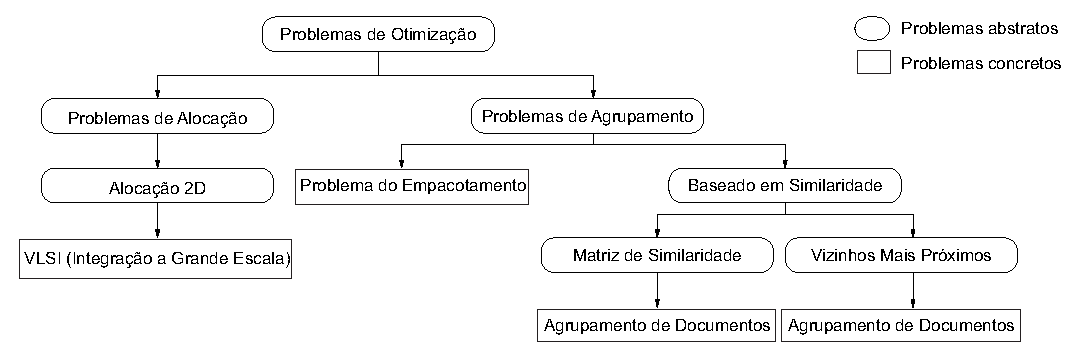
\includegraphics[width=1.0\textwidth]{problemasDeOtimizacao.eps}
%	\caption{Some Optimization Problems.\commentib{Falta apenas traduzir a imagem.} \label{fig:problemasDeOtimizacao}}
%	\end{figure*}
%	
%	An optimization problem can be defined as a finite set of variables, where the correct values for the variables specify the optimal solution. If the variables are of the set of real, the problem is called continuous, and if they can only have a finite set of distinct values, the problem is called combinatorial \protect\cite{francq2011optimization}.
%	
%	In order for the optimization problems to be solved, it is necessary to develop a method that solves them, which are the algorithms. An important category of problems are the NP-hard problems, where they can only be solved by certain algorithms that try to arrive at the optimal solution of that determined problem.
%	
%	When the optimal solution of an NP-hard problem is not guaranteed, this type of method is called a heuristic. A heuristic is an intuitive way of solving a particular problem, where the best possible solution is not guaranteed.
%	
%	Every optimization problem is basically characterized by having an objective function, which can be called cost function when it is desired to minimize it or utility function when it is desired to maximize it, and a set of constraints that delimit the space of viable solutions, or Be the region where the solutions are that can be accepted. The objective function contains a set of variables to which values must be assigned in a systematic way so as to walk through the search space and find the one that optimizes the result to be searched, in case a maximization problem finds the highest possible value while in a Minimize the value. In both cases the solution must satisfy the set of constraints imposed to be accepted. 


%	One can interpret the space of solutions as being a subset of Euclidean space \(\R^n\). Each variable is a dimension of space. For a function with two variables it is possible to form in a two-dimensional space and with the addition of a third dimension to the result of the function with \(x\) and \(y\) as input it is possible to observe the behaviour of the function as The \(x\) and the \(y\) of the function undergo variation. In Figure ~\ref{fig:sol} a two-dimensional graph is shown in which the variation of the function value causes changes in the gray scale. For larger values ??a darker gray is obtained and for smaller values ??a lighter gray is obtained. With this, one can observe the space of solutions in a panoramic way in the two-dimensional space and it is verified that as it approaches the center the function generates smaller values. In it it is also possible to notice that the x-shaped marks, which represent the solutions found, vary towards the local minimum that is in the middle of the search space. The heuristic used to search for the optimal solution in this case was to look for neighbouring solutions that minimized the cost of the function in the same way that a sphere that rolls over an inclined plane stabilizes when it reaches a valley that would be the local minimum Function. However, this heuristic is not always the most adequate, as will be seen later.
%
%\begin{figure}[H]
%	\centering
%	\includegraphics[width=0.5\textwidth]{sol.eps}
%	\caption{Walking through the space of solutions\label{fig:sol}}
%\end{figure}

%%%%%%%%%%%%%%%
\section{UAV Movement System}
\label{sec:uav}
%%%%%%%%%%%%%%%

% \subsection{UAV Movement System}

In this section, we first investigate the platform used in this work, verifying the hardware characteristics and how to control it by software. The core hardware of the UAV IRIS+ is the Pixhawk and we can control it using a Python library - dronekit that uses MAVLink\footnote{MAVLink or Micro Air Vehicle Link is a protocol for communicating with small unmanned vehicle. It is designed as a header-only message marshalling library} protocol. Secondly, we integrate a robot gripper to the UAV to take and leave packages during the mission. After that, we created movement functions to make the UAV movement and control it using some resources of the dronekit API.
\begin{figure}[H]
	\centering
	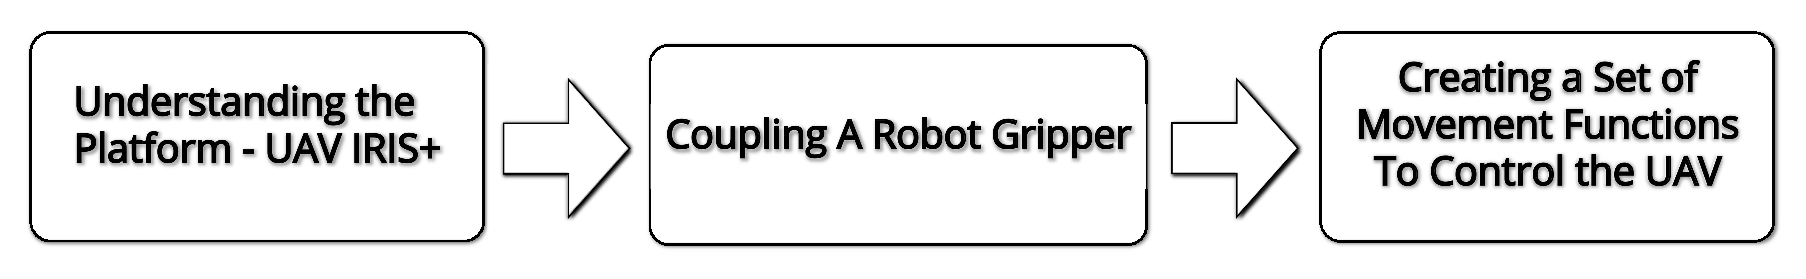
\includegraphics[width=0.25\textwidth]{movement.eps}
	\caption{UAV Movement Systems. \commentib{Vc poderia refazer a figura na horizontal para ocupar menos espa\c{c}o?} \label{fig:movement}}
\end{figure}

\commentib{Fale um pouco mais aqui...}

%\subsection{Mission Planning}
%\label{mission}


%%%%%%%%%%%%%%%
\section{Methodology of Time Cost Evaluation, UAV use and Mission Planning}
\label{sec:method}
%%%%%%%%%%%%%%%

%\commentib{Modifique o t\'itulo (expanda). Metodologia de qu\^e?? Tente fazer algo parecido com o do trabalho.}

	%In this section, there will have a brief clarification of the contents of this paper.

\commentib{outline here}

%%%%%%%%%%%%%%%
\subsection{Modeling an UAV Intralogistics Mission as an Optimization Problem }
\label{ssec:modelo}
%%%%%%%%%%%%%%%



%The purpose of this subsection is to elaborate a modelling of the mission planning problem in an optimization problem. In order to find later, the shortest execution time of all the tasks (minimization), based on the data below:

It is assumed that the processing time $ p_i $ is the total time of production of $i$-th \commentib{dizer aqui o significado do \'indice $i$}, that is the time demanded to leave and take \commentib{quais produtos??} products, considering the sum of the time that the UAV stays in the stock collecting inputs and the time that demanded for the UAV movement. We also assume that the setup (production) time $s_i$ is the time required only for the manufacturing of a product, considering that all the required inputs are available in the production line. Therefore, the total time for the production of a given product is the sum of the processing  and setup time ($p_i$  and$s_i$).

\textcolor{red}{ The fictive task or dummy of the scheduling, $j_0$, with processing time proportional to the time that the UAV collect the input and leads to the production line.}\commentib{Reescrever frase anterior} In the literature, production lines are called considered parallel machines \commentib{diga o que \'e isso} for optimization problems of scalable tasks (when there are $m$ machines in parallel with performances depending on the task to be executed, notation used is $R$ \commentib{explique melhor o que est\'a nesse par\^entese e tire do par\^entese}) \cite{du2008scheduling}.

\paragraph{Model variables} To obtain a model for our UAV intralogistics mission planning problem, we must consider the following variables:
\begin{itemize}
\item $\mathcal{T} = \set{T_j \vert j\in \mathbb{N}^{*},i\leq N}$ is the set of $N$ tasks;
\item $\mathcal{M} = \set{m_i \vert i\in \mathbb{N}^{*},i\leq M}$ is the set of $M$ machines (production lines);
\item $\mathcal{P} = \set{p_j \vert j\in \mathbb{N}^{*},i\leq N}$ is the processing time of each $j$-th task;
\item $S = \set{s_i \vert s\in \mathbb{N}^{*},i\leq M}$  is the setup (production) time of each $i$-th production line;
\item $R||C_{max}$ (Three-field notation\footnote{Notation $\alpha | \beta | \gamma$, where $\alpha$: processing environment, $\beta$: problem constraints and $\gamma$: optimization criterion.} used in the literature to represent a given task scheduling problem, in this case, minimizing the makespan \footnote{Makespan is the termination time of the most loaded processor.} in an unrelated parallel machine environment \cite{graham1979optimization}. \commentib{Isso \'e necess\'ario msm? N\~ao parece ser usado em nenhum lugar.}
\end{itemize}	

\paragraph{Objective function}

The objective function is the variable $C_ {max}$ (total process execution time) that needs to be minimized.
\begin{equation}
	\begin{array}{cc}
		\min & C_{max}  \\
	\end{array}
\end{equation}
\commentib{Podemos modelar de alguma forma o $C_{max}$?}

\paragraph{Constraints}

The binary variable $x_ {ij}$ is equal to $1$ if and only if the task $j$ is running on the machine $i$, and $0$ otherwise, {\it i.e.}, $x_ {ij}$ is defined as follows:
\begin{equation}
\begin{split}
x_{ij}=\begin{cases}
    1,       & \quad \text{if the task } j \text{ is running in} \\
 &\text{ the machine }i\\
    0,  & \quad \text{otherwise}\\
  \end{cases}
\end{split}
\end{equation}

The first constraint related to our intralogistics mission planning optimization problem is related to the exclusivity execution of a task, {\it i.e.}, each task must be executed/processed in an unique machine:
\begin{equation}
\sum_{i=1}^{M}{\sum_{j=1}^{N}{x_{ij}}}=1
\end{equation}

% For a better understanding what the summation means, let's suppose that there are two production lines and tree products to be produced (tasks), therefore, $x_{00}+x_{10}+x_{20}=1$, $x_{01}+x_{11}+x_{21}=1$ and $x_{02}+x_{12}+x_{22}=1$, so, it can be verified that those restrictions are set, there will be only one task running in a machine.

\paragraph{Resulting optimization problem}
{\color{red}
Model:

\begin{enumerate}
\item \textbf{Choosing the constraints:}



\begin{equation}
C_{max}=makespan \text{ (duration of a mission)}
\end{equation}
\item \textbf{Elaboration of the objective function:}
The objective function is the variable $C_ {max}$ (total process execution time) that needs to be minimized.
\begin{equation}
\text{Minimize } C_{max}
\end{equation}
$C_{max}$ is the variable that need to be minimized (optimized).
\item \textbf{Restrictions:}

\begin{itemize}
\item \textbf{Each task must be executed/processed in an unique machine (production line)}

\begin{equation}
\sum_{\substack{
   i \in M\\
   \forall j \in J
  }} 
 x_{ij}=1
\end{equation}

For a better understanding what the summation means, let's suppose that there are two production lines and tree products to be produced (tasks), therefore, $x_{00}+x_{10}+x_{20}=1$, $x_{01}+x_{11}+x_{21}=1$ and $x_{02}+x_{12}+x_{22}=1$, so, it can be verified that those restrictions are set, there will be only one task running in a machine.

\item \textbf{Time execution of the tasks in each machine}

\begin{equation}
\sum_{\substack{
   j \in J\\
   \forall i \in M
  }} 
 (p_j+s_j)x_{ij}\leq C_{max}
\end{equation}

For a better understanding what the summation means, let's suppose that there are two machines and two tasks, and the time of processing and setup of each task are $p_0=100,~ p_1=100$ and $s_0=12,~ s_1=18$ respectively. Therefore, the production time of the product $0$ in the production line $0$ is $p_0 + s_0$ and so on. 
\end{itemize}
\item \textbf{Completeness and non-negativity:}

\begin{equation}
\begin{split}
 x_{ij} \in \{0,1\}~\forall i=1,2,...,M\text{ and }\\
 \forall j=0(dummy), 1,2,3,...,N
\end{split}
\end{equation}

\item \textbf{Full model:}
\begin{align*}
\begin{split}
\text{Minimize~~~}  & C_{max} \\
    \text{Subject to~~~}  &\sum_{\substack{
   i \in M\\
   \forall j \in J
  }} 
  x_{ij}=1 \\
    & \sum_{\substack{
   j \in J\\
   \forall i \in M
  }} 
 (p_j+s_j)x_{ij}\leq C_{max} \\
 	& x_{ij} \in \{0,1\}~\forall i=1,2,...,M ~e~
 	\forall \\
 &j=0(dummy), 1,2,3,...,N
\end{split}
\end{align*}

\end{enumerate}
}
%%%%%%%%%%%%%%%
\subsection{Planner Evaluation Methodology}
\label{ssec:evaluationmethod}
%%%%%%%%%%%%%%%

The main contribution of this work is a methodology to evaluate UAV mission planner algorithms and find minimum cost planner. To this purpose, a generalized evaluation metric is developed. The objective (cost) function modeled in Section \ref{ssec:modelo} is related to the total tume spent for the execution of the mission. Our evaluation metric compares the cost of a planner algorithm with the best cost computed by the CPLEX \commentib{1 REF} solver. The metric presented here will be called Mission Planner Cost Index ($MPCI$).

Firstly, the optimal cost of the problem is obtained through the CPLEX solver, which returns the optimum value (minimum mission execution time). The optimization problem is modeled with C++ {\color{red} with the aid of the CPLEX solver} \commentib{Como assim? Diga como o CPLEX ajuda a modela o problema em C++}. 

\commentib{Voc\^e deve deixar claro como o $c_X$ \'e calculado. O texto n\~ao fala sobre isso. Escreva nesse par\'agrafo}


Finally, the evaluation of each mission planner is computed with relation to the optimal cost, therefore, the $MPCI_{X}$ of a planner $X$ is computed as follows:
\begin{equation}
	MPCI_X=\frac{c_o}{c_X},
\end{equation}
where $c_o$ is the optimal cost obtained by the CPLEX solver, \textbf{$c_X$} is the cost of the olution generated by planner $X$, and $0 \leq MPCI_X \leq 1$. Note that as close of $1$ the $MPCI_X$ is, the solution cost is smaller.

%%%%%%%%%%%%%%%%%%%%%%%%%%%%%%%%%%%%%
\section{Experimental Evaluation}
\label{sec:results}
%%%%%%%%%%%%%%%%%%%%%%%%%%%%%%%%%%%%%
 
%%%%%%%%%%%%%%%%%%%%%%%%%%%%%%%%%%%%%
\subsection{Experimental Environmental and Objectives}
\label{ssec:expobjandenv}
%%%%%%%%%%%%%%%%%%%%%%%%%%%%%%%%%%%%% 
 
\commentib{completar} 
 
%%%%%%%%%%%%%%%%%%%%%%%%%%%%%%%%%%%%%
\subsection{Case Study}
\label{sec:ec}
%%%%%%%%%%%%%%%%%%%%%%%%%%%%%%%%%%%%%

To demonstrate the use of the methodology of evaluation of UAV mission planners for intralogistics missions, the case study shown in Figure~\ref{fig:useCase} is used.

\begin{figure}[ht]
	\centering
	\includegraphics[width=0.45\textwidth]{useCase.eps}
	\caption{Case Study Representation \commentib{traduzir figura e numerar/nomear linhas de produ\c{c}\~ao}.\label{fig:useCase}}
\end{figure}
	
Figure~\ref{fig:useCase} shows that there are three types of inputs in the warehouse ({\it i.e.}, A, B, and C) and two production lines that produces two different products ({\it i.e.}, X and Y). Each production line produces only one type of product and has a characteristic production time.  Figure~\ref{fig:useCase} shows that to produce a product of type X, two inputs of type A and one input of type C are required, and to produce a product of type Y, two inputs of type B and one input of type C are required. The production time of a X product is $4 p.u.$ and the time of production of product Y is $6 p.u.$. A production unit ($1 p.u.$) was considered to be a \texttt{GoTo} command performed by the UAV. \commentib{O leitor n\~ao vai ter ideia do que \'e um goto. Tem que tido uma explica\c{c}\~ao sobre isso em algum lugar l\'a atr\'as.}

The task to be performed is the production of the customer order, where the UAV will collect supplies from the warehouse, take to the production line and once the production of a certain product is finished, it will lead to the customer.

\subsection{Mission Planners}

In this work, we considered that mission planner is a software that generates a production mission given the warehouse and customer order. This program generates a \texttt{.mission} extension file containing a set of mission commands, as shown in the~\ref{mission} subsection. \commentib{o leitor tb n\~ao saber\'a o que \'e esse .mission}. Two examples of planners are presented in this work and will be employed to demonstrate the cost evaluation methodology.

\subsubsection{Planner A}

{\color{red}
In this strategy, the UAV starts moving toward the warehouse, takes two inputs of type A to produce a product X, then takes the type C input, waits on the production line for the product X to be produced. After being produced, it leads to the customer. If there is more products of type X to be produced, it goes to the warehouse and carries out the whole process again.

After all the X products are produced and taken to the customer, the UAV will go to the warehouse and take the two type B inputs and then the type C input, wait for the first product Y to be produced and then take it to the customer. If you need to produce more Y products, the process is the same.}

\commentib{Acho que o texto n\~ao est\'a bem explicado e est\'a longo. Voc\^e consegue resumir e melhorar a explica\c{c}\~ao?}

The general steps of planner A are shown in the Algorithm~\ref{alg:planA}.

\begin{algorithm}[ht]
\footnotesize
\KwIn{warehouse}
\KwIn{order}
\KwOut{mission file \textit{.mission}}
\Begin{
check the order\;
\Repeat{production of all X elements finish}{
go to the warehouse}\;
\Repeat{until bring 2 A elements}{
	get input A\;
	bring to the production line X\;
}
go to the warehouse\;
get the input C\;
bring to the production line X\;
wait X to be produced\;
bring X to the client\;

\Repeat{production of all Y elements finish}{
go to the warehouse\;
\Repeat{until bring 2 B elements}{
	get input B\;
	bring to the production line Y\;
}
go to the warehouse\;
get the input C\;
bring to the production line Y\;
wait Y to be produced\;
bring Y to the client\;
}
}
\captionsetup{list=no}
\caption{Planner A}\label{alg:planA}
\end{algorithm}

\subsubsection{Planner B}
In planner B, unlike planner A where the UAV is idle waiting for each product to be produced and only then takes the customer, the UAV continues the production process while the output of the products does not end. Once the production of each product is finished, {\color{red} the UAV for the task that was running and goes to the production line of that particular product} \commentib{tem algo estranho nesse trecho... o que vc quis dizer?}, performs the collection and takes it to the customer. It then returns the task it was previously running, performing a scheduling of tasks.

The general steps of planner B are shown in the Algorithm~\ref{alg:planB}:

\begin{algorithm}[ht]
\footnotesize
\KwIn{warehouse}
\KwIn{order}
\KwOut{mission file \textit{.mission}}
\Begin{
initialize $t_x$\;
initialize $t_y$\;
check the order\;
\Repeat{production of all X elements finish}{
\uIf{the counter of that X is not $t_x$}{
go to the warehouse\;
\Repeat{until bring 2 A elements}{
	get the input A\;
	bring to the production line X\;
}
go to the warehouse\;
get the input C\;
bring to the production line X\;
start the counter of this X (production time)\;
keep producing\;
}
\Else{go back to the production line X\;
		bring X to the client\;
		go back to producing\;}
}
\Repeat{production of all X elements finish}{
\uIf{the counter of that X is not $t_y$}{
go to the warehouse\;
\Repeat{until bring 2 B elements}{
	get the input B\;
	bring to the production line Y\;
}
go to the warehouse\;
get the input C\;
bring to the production line Y\;
start the counter of this Y (production time)\;
keep producing\;
}
\Else{go back to the production line Y\;
		bring X to the client\;
		go back to producing\;}
}
}
\captionsetup{list=no}
\caption{Planner B}\label{alg:planB}
\end{algorithm}

\subsection{Cost Evaluation}
\label{ssec:acusto}

After the implementation of the algorithm of planners A and B, the metric shown in this work was used to evaluate the cost of the algorithms. The results of the proposed mission planning methods in this work were compared to the optimal solution obtained with the branch-and-cut algorithm of the IBM/ILOG CPLEX 12.4 tool developed in C++.

In order to obtain better results in the comparison, it was considered only the time in which the UAV takes to finish the production of a product, excluding the time in which it leaves its initial position and moves to the warehouse, the time in which it Moves from the customer to the warehouse and the time it takes to go to the end point and land. This was done due to the greater practicality of implementing the problem in the CPLEX solver. The problem was modelled considering the total processing time, that is, only the processing time of the task (production) and the time of set-up (time of production of the line). Thus, the execution time of each mission was measured and compared to the value obtained by the CPLEX solver (optimal time), as shown in Table~\ref{fig:comp}.

\begin{table}[H]
\centering
\begin{tabular}{@{}
>{\columncolor[HTML]{FFFFFF}}c 
>{\columncolor[HTML]{FFFFFF}}c @{}}
\cmidrule(l){2-2}
                      & \textbf{Time (s)}    \\ \midrule
\textbf{Planner A} & 420					  \\
\textbf{Planner B} & 404                   \\
\textbf{CPLEX}        & 134                   \\ \bottomrule
\end{tabular}
\caption{Time execution for comparison with the optimal solution time}
\label{fig:comp}
\end{table}

The Table~\ref{fig:comp} shows the mission execution times obtained using the scheduler algorithm A, the scheduler algorithm B, and the minimum value given by the solver.

Using the metric shown in the section~\ref{sec:ac}, then:

\begin{equation}
Creal_A=\frac{134}{420}=0,319
\label{eq1}
\end{equation}

\begin{equation}
Creal_B=\frac{134}{408}=0,328
\label{eq2}
\end{equation}

It can be seen in the Equation~\ref{eq2} that planner B performs the mission more quickly and has a lower cost than planner A, according to the metric used.

\subsection{Practical Results}

To verify the practical results, as well as a cost comparison between the different approaches of mission planners developed in this work, the flight time measurement was performed using the two mission planning algorithms developed, using the case study shown in \ref{sec:ec}.

Below, we can verify the two mission files generated by the two strategies developed in this work:

%\begin{figure}[H]
%\centering
%\begin{subfigure}{.5\textwidth}
%  \centering
%  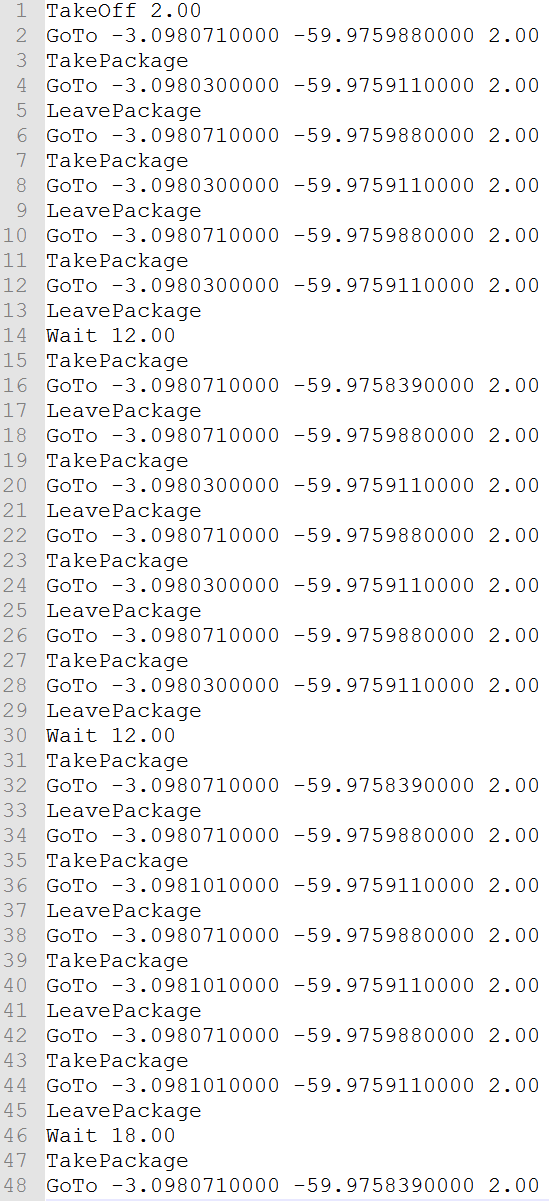
\includegraphics[width=.6\linewidth]{planAArq.PNG}
%  \caption{Planejador A.}
%  \label{fig:planAArq}
%\end{subfigure}%
%\begin{subfigure}{.5\textwidth}
%  \centering
%  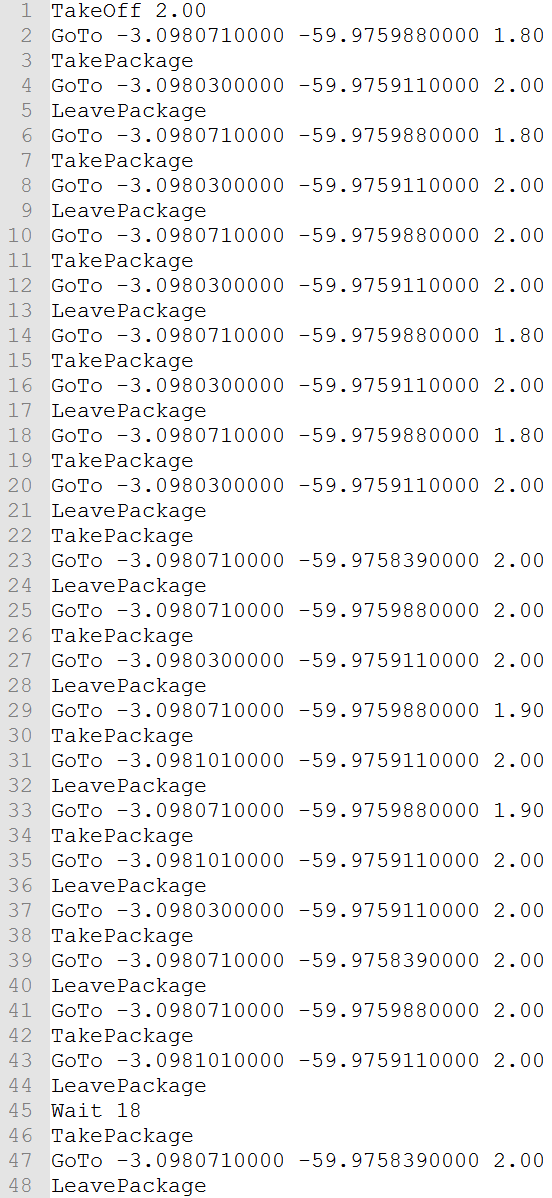
\includegraphics[width=.6\linewidth]{planBArq.PNG}
%  \caption{Planejador B.}
%  \label{fig:planBArq}
%\end{subfigure}
%\caption{Arquivos de Missão.}
%\label{fig:planArq}
%\end{figure}

%The two mission files shown above, have exactly the same instances, that is, they have the same resources and have to perform the same mission that is to produce two products of type X and one of type Y. However, they execute the mission of Different way and have different performances. As discussed in Section~\ref{sec:acusto}, planner B has more \texttt{GoTo} commands than planner A (see Figure~\ref{fig:planArq}).

The following is data about the mission being executed in the simulator SITL \footnote{Simulator that allows executing a Plane, Copter or Rover without the need of a hardware)}. The table below shows the performances of both schedulers relative to flight time.

\begin{table}[H]
\centering
%\begin{adjustbox}{max width=\textwidth}
\resizebox{7cm}{!}{%
\begin{tabular}{@{}ccc@{}}
\cmidrule(l){2-3}
                                        & \cellcolor[HTML]{FF7774}\textbf{Planner A} & \cellcolor[HTML]{5FCE89}\textbf{Planner B} \\ \cmidrule(l){2-3} 
\cellcolor[HTML]{C0C0C0}\textbf{Testes} & \textit{\textbf{Flight Time (s)}}            & \textit{\textbf{Flight Time (s)}}            \\
\cellcolor[HTML]{C0C0C0}1               & 460,405                                       & 430,830                                       \\
\cellcolor[HTML]{C0C0C0}2               & 460,693                                       & 436,885                                       \\
\cellcolor[HTML]{C0C0C0}3               & 462,080                                       & 441,681                                       \\
\cellcolor[HTML]{C0C0C0}4               & 457,719                                       & 441,277                                       \\
\cellcolor[HTML]{C0C0C0}5               & 461,227                                       & 451,865                                       \\ \bottomrule
\end{tabular}%
}
%\end{adjustbox}
\caption{Mission Planners Flight Time - Simulator.\label{table:plannersSimulado}}
\end{table}

In the Table~\ref{table:plannersSimulado}, it can be verified that the mission time executed by planner B presented less time compared to planner A in all five tests.

In Figure~\ref{fig:GraPlannersSimulado} is shown a graph of the flight times of both planners in the five tests done in the simulation environment.

\begin{figure}[H]
	\centering
	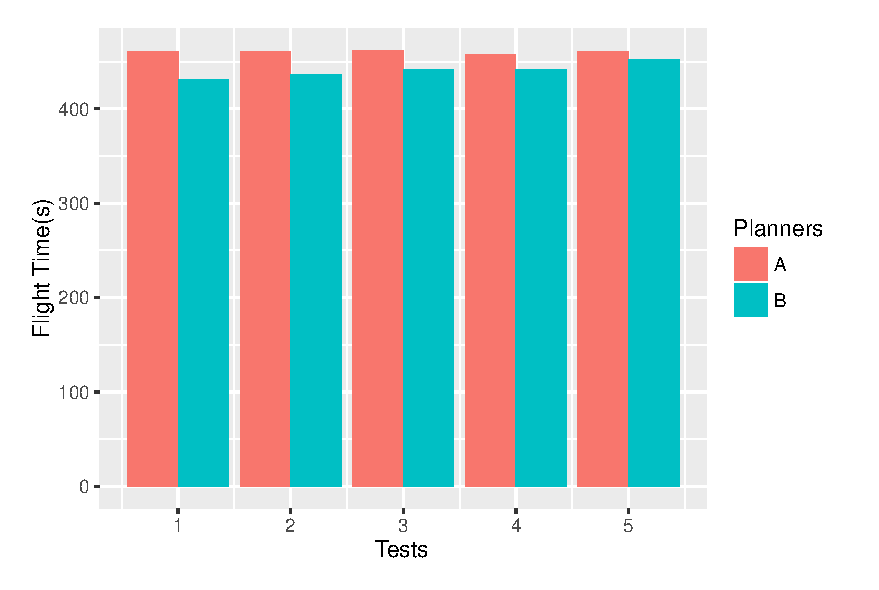
\includegraphics[width=0.5\textwidth]{GraPlannersSimulado.eps}
	\caption{Flight Time Graph of Mission Planners Relative to 5 Tests in Simulator.\label{fig:GraPlannersSimulado}}
	\end{figure}
	
	Next, you can see the results for the tests performed in real environment used by both planners.
	
	In Figure~\ref{fig:maps} the map where the tests were performed is shown on the map at the Faculty of Physical Education and Physiotherapy of Federal University of Amazonas.
	
		\begin{figure}[H]
	\centering
	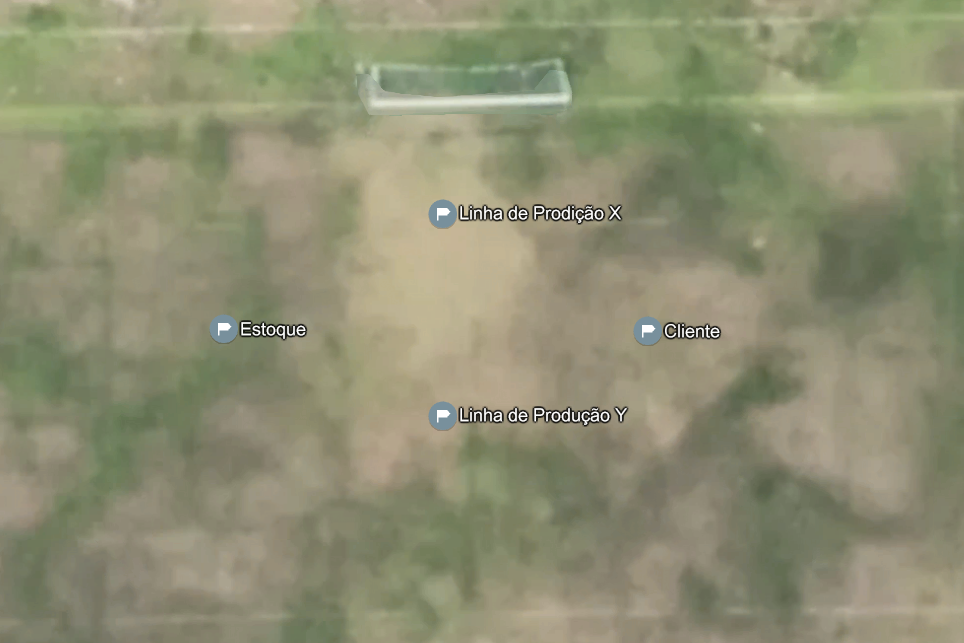
\includegraphics[width=0.47\textwidth]{mapsUseCase.PNG}
	\caption{Warehouse, Production Line X, Production Line Y and Costumer in the Map.\label{fig:maps}}
	\end{figure}
	
	In Table~\ref{table:plannersReal}, it can be seen that the mission time executed by planner B in real environment also showed a shorter time compared to planner A in the five tests:
	
	\begin{table}[H]
\centering
\resizebox{7cm}{!}{%
\begin{tabular}{@{}ccc@{}}
\cmidrule(l){2-3}
                                        & \cellcolor[HTML]{FF7774}\textbf{Planner A} & \cellcolor[HTML]{5FCE89}\textbf{Planner B} \\ \cmidrule(l){2-3} 
\cellcolor[HTML]{C0C0C0}\textbf{Testes} & \textit{\textbf{Flight Time (s)}}            & \textit{\textbf{Flight Time (s)}}            \\
\cellcolor[HTML]{C0C0C0}1               & 455,12                                       & 441,72                                       \\
\cellcolor[HTML]{C0C0C0}2               & 456,93                                       & 440,18                                       \\
\cellcolor[HTML]{C0C0C0}3               & 457,19                                       & 447,51                                      \\
\cellcolor[HTML]{C0C0C0}4               & 460,25                                       & 438,19                                       \\
\cellcolor[HTML]{C0C0C0}5               & 459.47                                       & 445,85                                       \\ \bottomrule
\end{tabular}%
}
\caption{Mission Planners Flight Time - Real.\label{table:plannersReal}}
\end{table}

In Figure~\ref{fig:GraPlannersReal} is shown a graph of the flight times of both planners in the five tests done in real environment.

\begin{figure}[H]
	\centering
	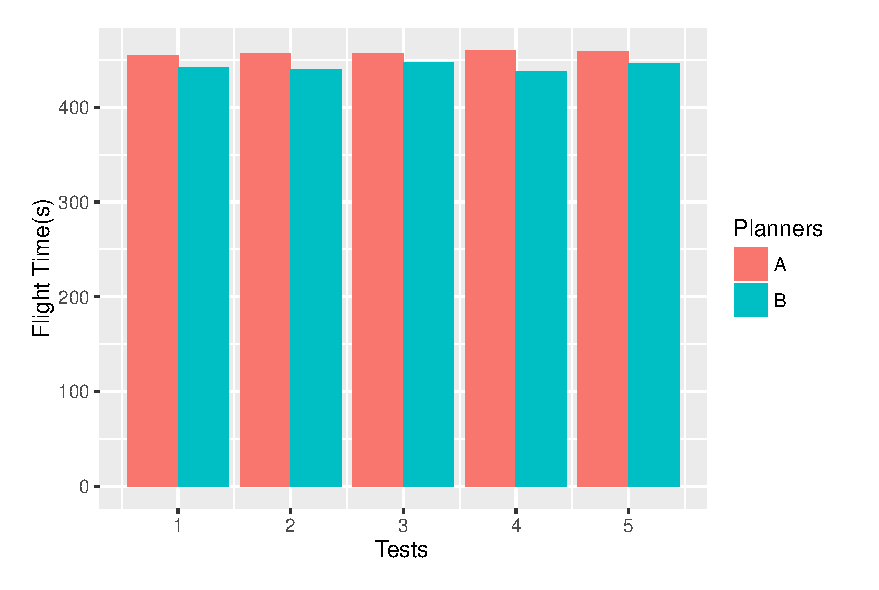
\includegraphics[width=0.5\textwidth]{GraPlannersReal.eps}
	\caption{Flight Time Graph of Mission Planners Relative to 5 Tests in a Real Environment.\label{fig:GraPlannersReal}}
	\end{figure}
	
	As shown in the section~\ref{sec:acusto}, planner B was faster than planner A. This can also be verified in real environment, as shown in tables \ref{table:plannersSimulado} and \ref{table:plannersReal} of mission execution time in simulated and real environment.

\section{Conclusions}
\label{sec:conclusao}

In this work, a common application of intra logistics performed by a VANT was developed, as well as the implementation of two mission planning strategies, as well as the cost evaluation of the same, compared to the optimal cost obtained by the CPLEX optimizer.

It is understood that some contributions were made with the conclusion of this work, such as:

In the manipulation and control of a commercial UAV, the ways of manipulating and controlling the 3DR IRIS + UAV of the UFAM Robotics Laboratory were investigated for future uses in undergraduate and postgraduate university projects.


Another important contribution was the creation of a methodology for evaluating the cost of mission planners, since it allows to verify their effectiveness against optimal values obtained by an optimizer.

Finally, it was possible to say that the manipulation and control of the 3DR IRIS+ UAV, as well as the creation of the cost evaluation methodology were successfully applied in simulated and real environments, thus validating the theory shown in the work.

Further works includes the use of computational vision for the recognition of inputs, improve the modeling of the optimization problem for better results in cost evaluation, and use a solver to directly generate an optimized mission.


%\selectlanguage{brazil}
%
%\section{Como utilizar o estilo \SBATeX}
%Este texto serve de guia de utilização do estilo \SBATeX para
%\LaTeXe. Com este estilo é possível gerar artigo no formato utilizado pelo \emph{Congresso
%  Brasileiro de Automática} e \emph{Simpósio Brasileiro de Automação Inteligente} na produção das versões acabadas dos artigos
%  nos anais.
%
%O seguinte parâmetro deve ser passado (entre colchetes) como argumento do comando
%\verb+\documentclass+, que deve ser o primeiro comando a aparecer no
%artigo. Por exemplo, o comando
%\begin{verbatim}
%  \documentclass[conference]{sbatex}
%\end{verbatim}
%é utilizado no início deste arquivo para geração do formato final
%para o \emph{Congresso Brasileiro de Automática} e o
%\emph{Simpósio Brasileiro de Automação Inteligente}.
%
%Pode-se adicionar ao comando \verb+\documentclass+ a seguinte
%opção:
%\begin{itemize}
%  \item \verb+harvard+: inclui o pacote \verb+harvard+, utilizado para
%  produção das referências bibliográficas. Pode ser usado em conjunto
%  com qualquer das outras opções. Veja seção~\ref{sec:bibliografia}.
%\end{itemize}
%Por exemplo, para propor um artigo ao congresso e utilizar o pacote de
%referências bibliográficas \verb+harvard+ usa-se o comando
%\begin{verbatim}
%  \documentclass[conference,harvard]{sbatex}
%\end{verbatim}
%A ordem dos parâmetros não é relevante.
%
%Os seguintes \emph{pacotes} \LaTeX\ estão disponíveis
%automaticamente\footnote{Isto também significa que \emph{é necessário
%ter estes pacotes instalados} para que se possa utilizar o estilo
%\SBATeX.} com o estilo \SBATeX:
%\begin{itemize}
%\item \verb+ifthen+: pacote com comandos de controle de fluxo do tipo
%`if', `then' e `else'; utilizado internamente para controle das opções de
%formatação.
%\item \verb+fancyhdr+: pacote para formatação dos cabeçalhos e rodapés.
%\item \verb+babel+: pacote para escrita em múltiplos idiomas; os
%idiomas/dialetos \verb+english+, \verb+brazil+ e \verb+spanish+ já
%estão habilitados.
%\item \verb+theorem+: pacote para controle dos ambientes \verb+theorem+,
%\verb+lemma+, \verb+corollary+ e \verb+proof+.
%\item \verb+geometry+: pacote para controle da dimensões do texto na página.
%\item \verb+latexsym+: pacote com símbolos extras do \LaTeXe.
%\end{itemize}
%
%A opção \verb+submission+ provê o pacote:
%\begin{itemize}
%\item \verb+setspace+: pacote para controle de espaçamento duplo entre
%linhas.
%\end{itemize}
%E a opção \verb+harvard+ provê o pacote:
%\begin{itemize}
%\item \verb+harvard+: pacote para formatação das referências
%bibliográficas.
%\end{itemize}
%
%Não é necessário incluir explicitamente as cláusulas
%\verb+\usepackage+ correspondentes a estes pacotes no artigo para que
%se possa utilizá-los. Caso a instalação do \LaTeX\ não contenha alguns
%destes pacotes, consulte a página
%\begin{verbatim}
%  http://www.ctan.org
%\end{verbatim}
%
%
%
%Com a opção \verb+conference+, e devido à escolha de um conjunto de
%fontes diferentes, recomenda-se subsituir o pacote \verb+fontenc+ pelo
%pacote \verb+ae+ (\emph{Almost European Computer Modern}), o que pode
%ser feito com o comando
%\begin{verbatim}
%  \usepackage{ae}
%\end{verbatim}
%Neste caso não é necessário adicionar explicitamente o pacote
%\verb+fontenc+, que já é carregado automaticamente pelo pacote
%\verb+ae+. Veja também a seção~\ref{sec:esqueleto}.
%
%Após o preâmbulo, inicia-se o texto propriamente dito por meio do
%comando
%\begin{verbatim}
%  \begin{document}
%\end{verbatim}
%O passo seguinte é a declaração do título do artigo, autores e
%afiliações.
%
%\subsection{Título, autores e afiliações}
%
%O título do artigo é declarado por meio do comando \verb+\title+. Por
%exemplo, o título deste artigo foi gerado com o comando:
%\begin{verbatim}
%  \title{Artigo Exemplo}
%\end{verbatim}
%O título não deve conter agradecimentos, os quais devem aparecer em
%uma seção separada, no final do artigo.
%
%Em seguida, definem-se os autores com seus endereços eletrônicos e
%afiliações por meio dos comandos \verb+\author+ e
%\verb+\address+. Por exemplo, o nome e endereço do primeiro autor
%deste artigo, João da Silva, é introduzido por meio dos comandos:
%\begin{verbatim}
%  \author{João da Silva}
%         {jsilva@silva.com}
%  \address{Endereço do João e da Maria\\
%           Em algum lugar\\
%           Cidade, Estado, País}
%\end{verbatim}
%Note-se que o comando \verb+\author+ requer dois argumentos: o nome e
%o endereço eletrônico. Quebras de linha podem ser obtidas na afiliação
%por meio do comando~\verb+\\+. Segue-se, neste exemplo, a declaração
%do nome e afiliação do segundo autor:
%\begin{verbatim}
%  \author{Joaquim Pereira}
%         {jpereira@pereira.org}
%  \address{Endereço do Joaquim\\
%           Em algum lugar\\
%           Cidade, Estado, País}
%\end{verbatim}
%
%Em geral, para cada comando \verb+\author+ deve haver um comando
%\verb+\address+ correspondente, salvo o caso de compartilhamento
%de endereços. Neste caso, omite-se o comando \verb+\address+ para
%o segundo autor e indica-se o número do endereço que se deseja
%compartilhar como um parâmetro adicional do comando
%\verb+\author+. Por exemplo, o comando:
%\begin{verbatim}
%  \author[1]{Maria da Silva}
%            {maria@pereira.org}
%\end{verbatim}
%indica que a Maria da Silva utilizará o endereço de número 1, que
%corresponde ao endereço de João da Silva.
%
%Os autores seguintes possuem endereços independentes e são
%introduzidos da maneira convencional:
%\begin{verbatim}
%  \author{Pedro Manoel}
%         {pedro@pedro.com}
%  \address{Endereço do Pedro e do Rafael\\
%           Em algum lugar\\
%           Cidade, Estado, País}
%
%  \author{José Rodrigues}
%         {jose@rodrigues}
%  \address{Endereço do José\\
%           Em algum lugar\\
%           Cidade, Estado, País}
%\end{verbatim}
%
%Finalmente, o autor Rafael é definido como
%\begin{verbatim}
%  \author[3]{Rafael Pires}
%            {rafael@pires}
%\end{verbatim}
%o que indica que Rafael compartilha o endereço de número 3 com Pedro
%Manoel. Lembre-se de que, apesar de Pedro Manoel ser o autor de número
%4, o seu endereço é o de número 3, uma vez que a Maria já compartilha
%-- sem segundas intenções -- do mesmo endereço com o João.
%
%O comando
%\begin{verbatim}
%  \maketitle
%\end{verbatim}
%coloca o título e os autores no formato adequado.
%
%
%\subsection{Resumo, abstract e palavras-chave}
%
%Os artigos devem conter um resumo em português (ou espanhol) e em
%inglês. O ambiente para definição dos resumos, em qualquer idioma, é o
%\verb+abstract+. Para diferenciar os idiomas utiliza-se o comando
%\verb+\selectlanguage+, do pacote \verb+babel+. Por exemplo, a seqüência
%de comandos produz um \emph{Abstract} seguido de um \emph{Resumo}:
%\begin{verbatim}
%  \selectlanguage{english}
%  \begin{abstract}
%    Yossarian says, ...
%  \end{abstract}
%
%  \selectlanguage{brazil}
%  \begin{abstract}
%    O Largo da Sé ...
%  \end{abstract}
%\end{verbatim}
%
%As \emph{palavras-chave} devem ser definidas por meio do comando:
%\begin{verbatim}
%  \keywords{Exemplo, Ilustração}
%\end{verbatim}
%
%Deste ponto em diante selecione o idioma a ser utilizado e
%inicie o texto da sua contribuição.
%
%\textbf{IMPORTANTE:} Caso esteja se produzindo um texto com a
%opção \verb+conference+, colocam-se os comandos que vão de
%\verb+\maketitle+ a \verb+\keywords+ dentro de um ambiente
%\verb+twocolumn+. Isto é necessário para que os resumos sejam
%formatados em coluna simples\footnote{Como este arquivo está
%adaptado para utilizar o formato adequado para o \emph{Congresso
%Brasileiro de Automática} e o \emph{Simpósio Brasileiro de
%Automação Inteligente}, isto já está feito}. Veja
%seção~\ref{sec:esqueleto}.
%
%
%\subsection{Teoremas, lemas, corolários e provas}
%
%Quatro ambientes já se encontram pré-definidos no estilo \SBATeX. São
%eles
%\begin{itemize}
%\item \verb+theorem+: ambiente para teoremas.
%\item \verb+corollary+: ambiente para corolários.
%\item \verb+lemma+: ambiente para lemas.
%\item \verb+proof+: ambiente para provas.
%\end{itemize}
%Segue-se um exemplo de utilização destes ambientes:
%\begin{lemma}[Desigualdade Subtrativa]
%Em um espaço vetorial linear normado $\|x\| - \|y\| \leq \|x - y\|$
%para quaisquer vetores $x$, $y$.
%\end{lemma}
%\begin{proof}
%\begin{align*}
%\|x\| - \|y\| &= \|x - y + y\| - \|y\| \ \\
%              &\leq \|x - y \| + \|y\| - \|y\| \\
%              &= \|x - y\|.
%\end{align*}
%\end{proof}
%Este lema é produzido pela seguinte sequência de comandos:
%\begin{verbatim}
%  \begin{lemma}[Desigualdade Subtrativa]
%    Em um espaço vetorial linear ...
%  \end{lemma}
%  \begin{proof}
%    ...
%  \end{proof}
%\end{verbatim}
%
%Estes ambientes, com exceção do ambiente \verb+proof+, aceitam
%um parâmetro opcional que define um nome. No exemplo acima, o nome
%\emph{Desigualdade Subtrativa} foi produzido por meio deste argumento.
%
%
%\subsection{Bibliografia}
%\label{sec:bibliografia}
%
%As referências são reunidas ao fim do manuscrito, arranjadas
%alfabeticamente pelo primeiro autor e cronologicamente para cada
%autor.
%
%\textbf{IMPORTANTE:} Todas referências citadas devem aparecer em algum
%outro ponto do texto.
%
%As citações seguem um estilo autor/ano (o mesmo
%usado na revista {\em Automatica}). O pacote \verb+harvard+ (já
%incluído pelo \SBATeX) provê vários comandos para inclusão de
%citações. Dois dois mais utilizados são o tradicional \verb+\cite+ e o
%\verb+\citeasnoun+. Veja um exemplo:
%\begin{verbatim}
%  O resumo deste artigo é um trecho do
%  livro~\citeasnoun{serafim}. Já o abstract é
%  extraído de~\citeasnoun{catch22}.
%  Informações sobre o estilo bibliográfico
%  \verb+harvard+ encontram-se
%  em~\citeasnoun{harvard}. Os interessados
%  devem consultar referências adicionais
%  sobre \LaTeX~\cite{latex,%
%  latex:guide,latex:companion}.
%\end{verbatim}
%produz o trecho:
%
%\begin{em}
%  O resumo deste artigo é um trecho do
%  livro~\citeasnoun{serafim}. Já o abstract é
%  extraído de~\citeasnoun{catch22}.
%  Informações sobre o estilo bibliográfico
%  \verb+harvard+ encontram-se
%  em~\citeasnoun{harvard}. Os interessados
%  devem consultar referências adicionais
%  sobre \LaTeX~\cite{latex,latex:guide,latex:companion}.
%\end{em}
%
%Recomenda-se a utilização do programa BibTeX para gerar as suas
%referências ~\cite{latex,latex:guide,latex:companion}. Note-se que
%não é necessário definir o estilo bibliográfico com o comando
%\verb+\bibliographystyle+, pois o mesmo é definido automaticamente
%pelo estilo \SBATeX. Basta incluir o arquivo de bibliografias,
%neste exemplo o artigo \verb+exemplo.bib+ por meio do comando.
%\begin{verbatim}
%    ...
%
%    \bibliography{exemplo}
%
%  \end{document}
%\end{verbatim}
%Note-se que este comando deve ser colocado logo antes do
%encerramento do artigo, o que é feito pelo comando
%\verb+\end{document}+, de tal forma a garantir que a bibliografia
%seja o último item do artigo.
%
%
%\subsection{Esqueleto deste arquivo no formato \SBATeX}
%\label{sec:esqueleto}
%
%Este arquivo, adaptado para gerar o formato adequado para o
%\emph{Congresso Brasileiro de Automática} e o  \emph{Simpósio
%Brasileiro de Automação Inteligente}, faz uso da seguintes
%instruções:
%
%\begin{verbatim}
%\documentclass[conference,harvard,brazil,english]{sbatex}
%  \usepackage[utf8]{inputenc}
%  \usepackage{ae}
%
%    ...
%
%    \twocolumn[
%      \maketitle
%
%      \selectlanguage{english}
%      \begin{abstract}
%        Yossarian says, ...
%      \end{abstract}
%
%      \selectlanguage{brazil}
%      \begin{abstract}
%        O Largo da Sé ...
%      \end{abstract}
%
%      \keywords{Exemplo, Ilustração}
%    ]
%
%    ...
%\end{verbatim}
%
%
%\section{Contribuição deste artigo}
%
%\subsection{Os vinte e sete erros mais comuns (de uma lista de cem)}
%\label{sec:27erros}
%
%Erros gramaticais e ortográficos devem, por princípio, ser
%evitados. Alguns, no entanto, como ocorrem com maior frequência,
%merecem atenção redobrada. O primeiro capítulo deste manual inclui
%explicações mais completas a respeito de cada um deles. Veja os cem
%mais comuns do idioma e use esta relação como um roteiro para fugir
%deles~\cite{manual}.
%
%\begin{enumerate}
%\item ``Mal cheiro'', ``mau-humorado''. Mal opõe-se a bem e mau, a
%bom. Assim: mau cheiro (bom cheiro), mal-humorado
%(bem-humorado). Igualmente: mau humor, mal-intencionado, mau jeito,
%mal-estar.
%
%\item ``Fazem'' cinco anos. Fazer, quando exprime tempo, é impessoal:
%Faz cinco anos.~/~Fazia dois séculos.~/~Fez 15 dias.
%
%\item ``Houveram'' muitos acidentes. Haver, como existir, também é
%invariável: Houve muitos acidentes.~/~Havia muitas pessoas.~/~Deve
%haver muitos casos iguais.
%
%\item ``Existe'' muitas esperanças. Existir, bastar, faltar, restar e
%sobrar admitem normalmente o plural: Existem muitas esperanças. /
%Bastariam dois dias.~/~Faltavam poucas peças.~/~Restaram alguns
%objetos.~/~Sobravam idéias.
%
%\item Para ``mim'' fazer. Mim não faz, porque não pode ser
%sujeito. Assim: Para eu fazer, para eu dizer, para eu trazer.
%
%\item Entre ``eu'' e você. Depois de preposição, usa-se mim ou ti: Entre
%mim e você.~/~Entre eles e ti.
%
%\item ``Há'' dez anos ``atrás''. Há e atrás indicam passado na frase. Use
%apenas há dez anos ou dez anos atrás.
%
%\item ``Entrar dentro''. O certo: entrar em. Veja outras redundâncias:
%Sair fora ou para fora, elo de ligação, monopólio exclusivo, já não há
%mais, ganhar grátis, viúva do falecido.
%
%\item ``Venda à prazo''. Não existe crase antes de palavra masculina, a
%menos que esteja subentendida a palavra moda: Salto à (moda de) Luís
%XV. Nos demais casos: A salvo, a bordo, a pé, a esmo, a cavalo, a
%caráter.
%
%\item ``Porque'' você foi? Sempre que estiver clara ou implícita a
%palavra razão, use por que separado: Por que (razão) você foi?~/~Não
%sei por que (razão) ele faltou.~/~Explique por que razão você se
%atrasou. Porque é usado nas respostas: Ele se atrasou porque o
%trânsito estava congestionado.
%
%\item Vai assistir ``o'' jogo hoje. Assistir como presenciar exige a:
%Vai assistir ao jogo, à missa, à sessão.  Outros verbos com a: A
%medida não agradou (desagradou) à população.~/~Eles obedeceram
%(desobedeceram) aos avisos.~/~Aspirava ao cargo de diretor.~/~Pagou ao
%amigo.~/~Respondeu à carta.~/~Sucedeu ao pai.~/~Visava aos estudantes.
%
%\item Preferia ir ``do que'' ficar. Prefere-se sempre uma coisa a outra:
%Preferia ir a ficar. É preferível segue a mesma norma: É preferível
%lutar a morrer sem glória.
%
%\item O resultado do jogo, não o abateu. Não se separa com vírgula o
%sujeito do predicado. Assim: O resultado do jogo não o abateu. Outro
%erro: O prefeito prometeu, novas denúncias. Não existe o sinal entre o
%predicado e o complemento: O prefeito prometeu novas denúncias.
%
%\item Não há regra sem ``excessão''. O certo é exceção. Veja outras
%grafias erradas e, entre parênteses, a forma correta: ``paralizar''
%(paralisar), ``beneficiente'' (beneficente), ``xuxu'' (chuchu),
%``previlégio'' (privilégio), ``vultuoso'' (vultoso), ``cincoenta''
%(cinqüenta), ``zuar'' (zoar), ``frustado'' (frustrado), ``calcáreo''
%(calcário), ``advinhar'' (adivinhar), ``benvindo'' (bem-vindo), ``ascenção''
%(ascensão), ``pixar'' (pichar), ``impecilho'' (empecilho), ``envólucro''
%(invólucro).
%
%\item Quebrou ``o'' óculos. Concordância no plural: os óculos, meus
%óculos. Da mesma forma: Meus parabéns, meus pêsames, seus ciúmes,
%nossas férias, felizes núpcias.
%
%\item Comprei ``ele'' para você. Eu, tu, ele, nós, vós e eles não podem
%ser objeto direto. Assim: Comprei-o para você. Também: Deixe-os sair,
%mandou-nos entrar, viu-a, mandou-me.
%
%\item Nunca ``lhe'' vi. Lhe substitui a ele, a eles, a você e a vocês e
%por isso não pode ser usado com objeto direto: Nunca o vi.~/~Não o
%convidei.~/~A mulher o deixou.~/~Ela o ama.
%
%\item ``Aluga-se'' casas. O verbo concorda com o sujeito: Alugam-se
%casas.~/~Fazem-se consertos.~/~É assim que se evitam acidentes. /
%Compram-se terrenos.~/~Procuram-se empregados.
%
%\item ``Tratam-se'' de. O verbo seguido de preposição não varia nesses
%casos: Trata-se dos melhores profissionais.~/~Precisa-se de
%empregados.~/~Apela-se para todos.~/~Conta-se com os amigos.
%
%\item Chegou ``em'' São Paulo. Verbos de movimento exigem a, e não em:
%Chegou a São Paulo.~/~Vai amanhã ao cinema.~/~Levou os filhos ao
%circo.
%
%\item Atraso implicará ``em'' punição. Implicar é direto no sentido de
%acarretar, pressupor: Atraso implicará punição.~/~Promoção implica
%responsabilidade.
%
%\item Vive ``às custas'' do pai. O certo: Vive à custa do pai. Use
%também em via de, e não ``em vias de'': Espécie em via de extinção. /
%Trabalho em via de conclusão.
%
%\item Todos somos ``cidadões''. O plural de cidadão é cidadãos. Veja
%outros: caracteres (de caráter), juniores, seniores, escrivães,
%tabeliães, gângsteres.
%
%\item O ingresso é ``gratuíto''. A pronúncia correta é gratúito, assim
%como circúito, intúito e fortúito (o acento não existe e só indica a
%letra tônica). Da mesma forma: flúido, condôr, recórde, aváro, ibéro,
%pólipo.
%
%\item A última ``seção'' de cinema. Seção significa divisão, repartição,
%e sessão equivale a tempo de uma reunião, função: Seção Eleitoral,
%Seção de Esportes, seção de brinquedos; sessão de cinema, sessão de
%pancadas, sessão do Congresso.
%
%\item Vendeu ``uma'' grama de ouro. Grama, peso, é palavra masculina: um
%grama de ouro, vitamina C de dois gramas. Femininas, por exemplo, são
%a agravante, a atenuante, a alface, a cal, etc.
%
%\item ``Porisso''. Duas palavras, por isso, como de repente e a partir
%de.
%
%\end{enumerate}
%
%\subsection{Observação importante}
%
%Os erros de português porventura presentes neste artigo
%\begin{itemize}
%\item ou foram introduzidos propositalmente para deleite dos leitores
%atentos,
%\item ou não constam da lista da seção~\ref{sec:27erros}.
%\end{itemize}
%
%\section{Conclusões}
%Nada resta senão desejar-lhe boa sorte na preparação de seu artigo. Contamos com seu trabalho e sua presença no SBAI 2017 a ser realizado em Porto Alegre-RS.
%
%\section*{Agradecimentos}
%Mencione aqui seus agradecimentos as agências de fomento e colaboradores no trabalho.


\selectlanguage{english}
% BIBLIOGRAFIA
\bibliography{exemplo}
\end{document}
